
\chapter{Diskussion}\label{cha:disk}

I detta kapitel diskuteras projektets genomförande, resultat,
vidareutvecklingsmöjligheter och etiska aspekter.

Till att börja med vill vi säga att hur domänspecifika språk kan kombineras med
fysik inte var något vi visste när projektet startade. En stor del av arbetet i
början av projektet ägnades därför åt att försöka komma på olika sätt att
använda dem ihop med olika fysikaliska områden. Det gjordes många experiment
innan vi hittade ett sätt att skapa domänspecifika språk för fysik som var annat än
triviala implementationer av formler, till exempel att formlen för
rörelseenergi, $E_k = \frac{mv^2}{2}$, kan skrivas som \texttt{ek m v = m * v *
v / 2} i Haskell. Detta experimenterande ledde till att
vi såg en slags strategi för hur de kan kombineras, vilket blev den
metodik som beskrivs i avsnitt~\ref{sec:konstruktion}. Det vi vill poängtera är
med andra ord att det har varit oklart hur projektet skulle kunna föras
framåt eftersom det inte funnits någon tydlig väg att följa.

\section{Genomförandediskussion}

Under projektets genomförande har det gjorts flera val av teorier och metoder att använda. Självklart behöver inte dessa val vi gjorde vara de bästa. Därför kommer vi här att kritisera dem och föreslå andra möjligheter. Närmare bestämt kommer mötet med testgruppen, urvalet och Literate Haskell att diskuteras.

Det sätt återkopplingen gjordes under projektet kan kritiseras på flera sätt. För det första bestod testgruppen av enbart tre personer. För det andra hölls mötet under en ytterst kort tid, ungefär en timme. Mötet hade behövt vara längre för att låta testgruppen i lugn och ro arbeta igenom ett par kapitel, inklusive att följa med i programmeringen som gjordes i läromaterialet. För det tredje var vi inte tydliga med målet med återkopplingen, nämligen om de tyckte det var meningsfullt att lära ut fysik med hjälp av domänspecifika språk. Det gjorde att de heller inte kunde tänka på dessa frågor. Med tanke på dessa tre brister i återkopplingens genomförande är alla slutsatser dragna med den som stöd ytterst osäkra.

Det går även att kritisera hur urvalet av områden gick till under projektet. Dels kan det ha lett till att enbart två domänspecifika språk för fysik implementerades (dimensioner och partikelmekanik). Dels skedde urvalet ur implementatörens perspektiv (det vill säga  vårt) och inte ur användarens perspektiv (studenten som ska nyttja läromaterialet). Med det menar vi att områden valdes utifrån hur det implementationsmässigt hängde ihop, till exempel att matematisk analys är grunden till flera tillämpningar. Istället hade områden kunnat väljas utifrån de fysikaliska problem studenter ska lösa i Fysik för ingenjörer, till exempel block och talja eller momentjämvikt, och utifrån det utforma domänspecifika språk.

% De olika sätten att tänka vid val av
% områden skiljer sig åt och mest fokus under projektet har lagts på
% implementationsperspektivet. Visserligen gjordes enstaka försök att tänka på det
% andra sättet också, men vi tyckte det var svårt att skapa några domänspecifika
% språk på det sättet (se avsnitt~\ref{sec:lampligt}). Vi hade dock kunnat utforska
% detta tankesätt grundligare än vad vi gjort, istället för att avfärda det som
% ett svårare sätt att gå till väga.

Till sist kan vi kritisera den allmänna metoden som valdes för utformningen av läromaterialet, nämligen att skriva varje kapitel som en löpande text om hur ett domänspecifikt språk implementeras eller tillämpas. Nackdelen är att det blir en passiv inlärning, även om det till en viss utsträckning finns övningar och läsaren uppmuntras implementera koden parallellt. Literate Haskell har definitivt bidragit till dessa passiva tendenser. Literate Haskell är en programfil som är väldigt väl beskriven hur programmet fungerar, vilket leder till att man ser den som en text att läsa istället för ett program att köra och experimentera med. Under projektets genomförande hade det därför varit av intresse att undersöka alternativa sätt att utforma lärotexten som uppmuntrat ett mer aktivt lärande. Det hade till exempel kunnat vara att presentera idén bakom fysikaliska dimensioner, och sedan låta studenten själv skapa implementationen. En fingervisning i form av ett enkelt exempel på en möjlig lösning kan vara ett sätt att göra detta.

\section{Resultatdiskussion}\label{sec:res_disk}

Detta avsnitt inleds med en övergripande diskussion om det resulterande
läromaterialet och för vem läromaterialet kan vara relevant, för att sedan
övergå till en mer generell diskussion kring kombinationen av domänspecifika
språk och fysik.

I projektets mål och avgränsningar stod det att vi skulle börja med klassisk
mekanik, för att i mån av tid även behandla termodynamik och vågrörelselära. I avsnitt~\ref{sec:res_laromaterial} nämns att de tre grundläggande
områdena dimensioner, matematisk analys och vektorer är färdiga, samt de
komposita områdena partikelmekanik, gungbräda och krafter på lådor. Med andra
ord har mekanik påbörjats, men inte termodynamik eller vågrörelselära. Det som återstår enligt oss när det kommer till mekanik är att tillämpa de grundläggande områdena på
fler fysikaliska problem utöver gungbräda och krafter på lådor. Vi tror att de
tre grundläggande områdena som är färdiga räcker. Förutom fler tillämpningar kan
mer fördjupande områden implementeras, till exempel bevisföring, något som redan
påbörjats, se avsnitt~\ref{sec:res_laromaterial}.
%Det är dock värt att nämna att vi är mycket nöjda med det material som vi har producerat. Våra kapitel är väl avgränsade, utformade och implementerade på det sätt som vi anser att de bör.

En annan del av målet var att läromaterialet skulle vara lättillgängligt genom
sitt språkbruk, publicering på en hemsida och fri tillgång till källkoden.
Vi kan konstatera att de senare två har genomförts. Vi passar även på att
säga att vi tycker att en lättanvänd hemsida är trevligare att använda än
PDF-filer eftersom de inte har sidbrytningar, fasta sidmarginaler som använder
skärmutrymme, med mera. Detta är visserligen mindre detaljer, men tillsammans
påverkar de upplevelsen i stort. Vi
tycker även att språket i läromaterialet är någorlunda lättsamt då vi skriver
talspråkligt och vardagligt, och förklarar svårigheterna grundligt. Språket hade
dock kunnat vara vänligare. Till exempel beskriver vi olika koncept som
``väldigt enkla'' fastän läsaren kanske inte alls tycker det.

Vi knyter här även an till lärandeteorierna i avsnitt \ref{sec:arcs}, som nämnde interaktion och snabba belöningar. Vårt läromaterial har visserligen ingen interaktiv sida, men typsystemet i Haskell kan ändå fungera som en fingervisare när programmeraren gör rätt eller fel. Det går exempelvis inte att räkna med dimensioner på ett felaktigt sätt, och funktionskomposition fungerar endast om båda funktionernas typdefinitioner (typer på argument och returvärde) stämmer överens. När det kommer till snabba belöningar kan den glädje programmeraren ser när koden kompilerar ses som en sådan. Läromaterialet innefattar även strategiskt placerade roliga bilder för att ge impulsiva glädjereaktioner.

Läromaterialet kan vara relevanta för flera grupper. Visserligen är målgruppen datastudenter, och vi har personligen dragit nytta av det,
men vi tror att det kan vara relevant för fler än så, till exempel kan läromaterialet även vara intressant för fysiklärare. Fäldt nämnde att han
tyckte att det rigorösa tankesätt läromaterialet skolar in läsaren i kan vara
användbart även i traditionell fysikundervisning. Det kan därför vara intressant att undersöka hur ett sådant här läromaterial kan
integreras i undervisningen.

En del av projektets mål var att diskutera kombinationen av
domänspecifika språk och fysik. I de tre följande avsnitten diskuterar vi därför
läromaterialets fokus på matematik och Haskell istället för fysik, vilka
fysikaliska områden som var lämpliga att göra domänspecifika språk till samt om
det finns en pedagogisk nytta i att kombinera de två. Diskussionen är till
största del baserad på våra erfarenheter efter att ha implementerat ett flertal
domänspecifika språk relaterade till fysik, men de är även baserade på
uppfattningar från testgruppen och Fäldt.


\subsection{Om läromaterialets fokus på matematik och Haskell snarare än
fysik}\label{sec:fpf}

Målet med läromaterialet var att lära ut fysik på ett roligt och
lättförståeligt sätt. Dock syns det i resultatet,
avsnitt~\ref{sec:res_laromaterial}, att mest fokus lagts på att
förklara och lära ut matematik och Haskell. Det finns
flera anledningar till varför så är fallet.

Problemet med att prata om en egen implementation av fysik är att
fysik inte är ett helt eget område. Snarare kan fysik betraktas som en
kombination av tillämpad matematik, experimentering, och
problemlösning. Det blir därför naturligt att när den faktiska
implementationen av fysikaliska beskrivningar och lagar sker, så är
matematiken i centrum. Att fysik är tillämpad matematik illustreras i
figur~\ref{fig:xkcd}, som även visar mer generellt hur en kedja av
områden är tillämpningar av varandra.

\begin{figure}[tph]
  \centering
  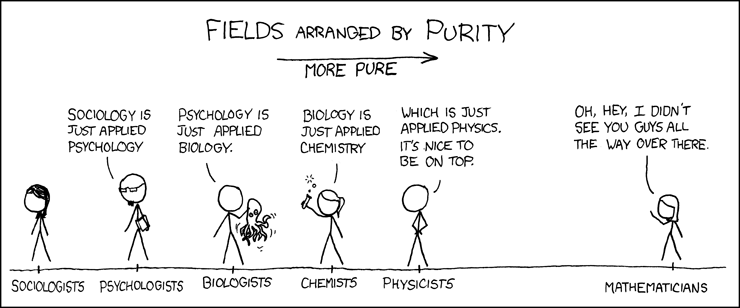
\includegraphics[width=0.9\textwidth]{figure/purity.png}
  \caption{\href{https://xkcd.com/435/}{Purity} (C) Randall Munroe (
  \href{https://xkcd.com}{xkcd.com}) \href{https://creativecommons.org/licenses/by-nc/2.5/}{CC BY-NC}. Bilden beskriver hur fysik är en tillämpning av matematik. Det är i själva verket
så att en kedja av områden kan betraktas som tillämpningar av
varandra.}\label{fig:xkcd}
\end{figure}

Anledningen till att stor fokus ibland läggs på Haskell är att de
koncept som används är viktiga för läsaren att förstå, men vi vill
förutsätta så lite förkunskaper som möjligt så att även oerfarna
Haskell-programmerare ska kunna följa med i boken. Ett syfte med
läromaterialet är också att väcka intresse hos läsaren, och vi tror
att detta kan uppnås genom att visa paralleller mellan funktionell
programmering, matematik, och implementationen av fysik.

Hade andra val gjorts i projektets tidigare skede, hade det kanske
sett annorlunda ut. Tidigt valde vi att söka efter områden som vi
ansåg vara fristående och väl avgränsade, se avsnitt~\ref{sec:valet},
och implementera dessa var för sig. Detta sätt att påbörja projektet
har påverkat allting som kom därefter. Om vi istället hade utvecklat
läromaterialet som en kombination av olika områden från början hade
det kanske inte varit lika främmande att även baka in problemlösning i
läromaterialet och på så sätt fått mer fysikorienterade domänspecifika
språk. Något annat som kan ha påverkat fokusen är valet av Haskell som
implementeringsspråk. Vi hävdar i teorikapitlet~\ref{sec:syntax} att
Haskells typer och fokus på mönstermatchning gör det idealt för
implementering av domänspecifika språk, men medför inte nödvändigtvis
att det är idealt för implementering av fysik. Det är möjligt att ett
annat språk eller till och med en annan paradigm hade lett till att
fokus hade hamnat på fysiken framför matematiken.

\subsection{Lämpliga områden för domänspecifika språk}\label{sec:lampligt}

När domänspecifika språk implementerades visade det sig att vissa områden lämpade sig bättre än andra. Exempel på ett lämpligt och ett mindre lämpligt område är vektorer respektive lutande plan\footnote{Läromaterialet behandlar fortfarande lutande plan, men inte som ett \textit{eget} domänspecifikt språk. Istället \textit{tillämpas} det domänspecifika språket för vektorer.}. Vad som skiljer dem åt är enligt oss att lämpliga områden består av tydliga \textit{data och operationer} medan mindre lämpliga områden består av \textit{egenskaper och samband}.

Inom området vektorer är vektorer data och till exempel vektoraddition en operation. I matematik defineras (en tvådimensionell) vektor som
\begin{align*}
  \vec{v} = \begin{bmatrix}
              v_1 \\
              v_2
            \end{bmatrix}
\end{align*}
och vektoraddition som
\begin{align*}
  \vec{u} + \vec{w} = \begin{bmatrix}
                        u_1 \\
                        u_2
                      \end{bmatrix}
                    + \begin{bmatrix}
                        w_1 \\
                        w_2
                      \end{bmatrix}
                    = \begin{bmatrix}
                        u_1 + w_1 \\
                        u_2 + w_2
                      \end{bmatrix}
\end{align*}
I Haskell kan en datatyp för vektorer defineras som
\begin{lstlisting}
data V = V Double Double
\end{lstlisting}
och vektoraddition som
\begin{lstlisting}
va :: V -> V -> V
(V u1 u2) `va` (V w1 w2) = V (u1+w1) (u2+w2)
\end{lstlisting}
Det finns enligt oss en tydlig likhet mellan matematik och Haskell i detta fall, och även i för andra lämpliga områden, vilket gör att vi tycker det blir enkelt att modellera och förstå områden som vektorer.

Egenskaper och samband är enligt oss svårare att modellera meningsfullt. Visserligen kan ekvationer modelleras i Haskell, men då blir det bara en ekvationslösare. Nyckeln, i till exempel lutande plan, är att känna till sambanden och veta när de ska användas. Vi behandlar därför lutande plan genom att tillämpa det domänspecifika språket för vektorer. Att vissa områden var mindre lämpliga var ett oväntat resultat. I början av projektets start trodde vi att domänspecifika språk skulle kunna implementeras till alla typer av områden.

\subsection{Domänspecifika språk, fysik och pedagogiska aspekter}\label{sec:bara_fysik}

En del av projektets mål är att diskutera huruvida det finns en pedagogisk nytta i att kombinera fysik och domänspecifika språk. Denna fråga diskuteras nedan.

I samband med fysik finns det några fördelar med att integrera domänspecifika språk. Domänspecifika språk kan betraktas som ``tools for thinking''\footnote{Uttryckt i Patrik Janssons egna ord, föreläsare i kursen DSLsofMath.} och ger ett nytt perspektiv på fysik och ger den \textit{struktur}. Dimensioner är ett exempel på detta, se avsnitt~\ref{sec:res_dim}. Där konstateras att en godtycklig dimension kan skrivas som de sju basdimensionerna med tillhörande exponenter, vilket kanske inte är så man brukar se på dimensioner, men som ger dem en väldefinierad struktur. Domänspecifika språk bidrar även med \textit{rigorösitet} till fysik. Enbart de definierade operationerna går att använda, vilket leder till att genvägar i fysikaliska beräkningar inte går att göra på det sätt som är möjligt vid räkning med papper och penna. Detta tyckte även Åke Fäldt var en bra aspekt, se avsnitt~\ref{sec:res_test}. Med hjälp av domänspecifika språk är det dessutom möjlighet att väcka \textit{intresse} för fysik. En student som inte är intresserad av fysik kanske skulle bli det om fysik presenteras i samband med Haskell och domänspecifika språk, där paralleller mellan dem visas. Denna tanke stöds även av testgruppen\footnote{Eftersom mötet med testgruppen var väldigt kort är det dock svårt att dra några säkra slutsatser.}, se avsnitt~\ref{sec:res_test}

År 2016 genomfördes ett kandidatarbete på Chalmers liknande
detta~\cite{kandidat2016}. Det kandidatarbetet resulterade också i ett
läromaterial, skillnaden är att det arbetet behandlade signallära. Grundidén är
dock densamma: att använda domänspecifika språk för att ge struktur till ett
annat område. Dessutom finns kursen \textit{Classical Mechanics: A Computational Approach}~\cite{classical-mechanics-course-mit-2008} som också använde domänspecifika språk till att ge struktur till fysik. Detta tycker vi visar på att det finns ett
akademiskt intresse för att använda domänspecifika språk i syfte att lära ut,
och att idén som vi presenterar i denna rapport även går att applicera på
andra områden. Nyttan att strukturera upp områden i väl avgränsade och
tydligt definierade delar kanske anses som uppenbar, men frågan om vilket
verktyg som ska användas för detta är inte lika uppenbar. Vi hävdar att
domänspecifika språk är ett sådant verktyg.

Det finns dock problem med att använda domänspecifika språk till att lära ut fysik. Ett problem är att den kreativa problemlösning som ingår är fysik är svår att fånga upp i domänspecifika språk\footnote{Enligt oss, och vi vet inte hur det skulle kunna göras.}. Ett annat problem är att det finns risk att fokus glider från fysik till domänspecifika språk. Ett läromaterialet om renodlad fysik med ett lättsamt språk och noggrann förklaring av koncepten hade säkert varit mycket uppskattat, det sätt som Khan Academy~\cite{khan} beskriver fysik är ett sådant exempel. En större målgrupp hade också kunnat nås då.

Avslutningsvis tror vi att domänspecifika språk med fördel kan integreras i traditionell fysikundervisning och på så sätt fånga upp de delar domänspecifika språk gör bra i fysik: strukturera, uppmuntra rigorös problemlösning och väcka intresse. Men samtidigt förlita sig på traditionella metoder till stor del i bland annat problemlösning och inte låta fokuset glida för långt från fysik till domänspecifika språk.

%En del av projektets mål är att diskutera huruvida det finns en pedagogisk nytta
%i att kombinera fysik och domänspecifika språk. Denna fråga diskuteras nedan.

%Domänspecifika språk kan betraktas som ``tools for thinking''\footnote{Uttryckt
%i Patrik Janssons egna ord, föreläsare i kursen DSLsofMath.}. Med det
%menas att domänspecifika språk kan användas till att strukturera ett område så
%att det blir enklare att få en överblick och
%förstå det. Dimensioner i läromaterialet är ett exempel på
%detta, se även avsnitt~\ref{sec:grund_impl}. Där konstateras att en godtycklig
%dimension kan skrivas som de sju grunddimensionerna med tillhörande exponenter.
%Det strukturerade sättet som dimensionerna sen beskrivs på ger förhoppningsvis
%ett enklare sätt att se på dem, vilket vi själva tycker är meningsfullt.

%År 2016 genomfördes ett kandidatarbete på Chalmers liknande
%detta~\cite{kandidat2016}. Det kandidatarbetet resulterade också i ett
%läromaterial, skillnaden är att det arbetet behandlade signallära. Grundidén är
%dock densamma: att använda domänspecifika språk för att ge struktur till ett
%annat område.

%\textbf{TODO: Hur fick det för den gruppen?}

%Detta tycker vi visar på att det finns ett
%akademiskt intresse för att använda domänspecifika språk i syfte att lära ut,
%och att idén som vi presenterar i denna rapport även går att applicera på
%andra områden. Nyttan att strukturera upp områden i väl avgränsade och
%tydligt definierade delar kanske anses som uppenbar, men frågan om vilket
%verktyg som ska användas för detta är inte lika uppenbar. Vi hävdar att
%domänspecifika språk är ett sådant verktyg.

%En annan aspekt är att när de domänspecifika språken används till fysikalisk
%problemlösning måste det ske enligt de regler som ställdes upp när de
%domänspecifika språken definierades. Det går med andra ord inte att fuska och ta
%genvägar i beräkningarna. Detta tankesätt tycker Fäldt, se
%avsnitt~\ref{sec:res_ake}, är en mycket bra aspekt som förmedlas med att
%presentera fysik på detta sätt. Studenten skolas in i att tänka i rigorösa och
%kompletta banor.

%Ett probem med användingen av våra domänspecifika språk är att problemlösining
%inte alltid är helt strukturerad och rigorös. Den kreativa problemlösning som en
%student kan utföra med papper och penna, utan att tänka på dimensioner och typer
%kan ej fångas upp med vår implementation, där misstag direkt straffas med
%kompileringsfel. Dock kan vår implementation vara behjälplig när en student väl
%ska testa sin lösning och vill ta reda på vilka misstag som gjorts.

%Hittills har domänspecifika språk framförts som ett sätt att strukturera fysik.
%Men läromaterialet har även haft två andra drag förutom domänspecifika språk,
%nämligen ett lättillgängligt språk och en noggrann genomgång av koncept.

%Genom att enbart ha fokus på fysik är det möjligt att fysiken i sig förklarats
%bättre än vad den gör nu. Ett läromaterial om renodlad fysik med ett lättsamt
%språk och noggrann förklaring av koncepten hade säkert varit uppskattat, det
%sätt som Khan Academy behandlar fysik är ett sådant exempel~\cite{khan} som är
%mycket uppskattat. En annan fördel hade varit att en större målgrupp kan nås.
%Men då förlorar vi de saker domänspecifika språk bidrar med, nämligen det som
%diskuterats ovan: att ge struktur och att lära ut ett rigoröst tankesätt.
%Även relevansen och den \textit{intresseväckande}
%potentialen kan förloras för datastudenter om programmeringsaspekterna
%försvinner från läromaterialet. Denna
%tanke stöds även av att testgruppen tyckte läromaterialet var ett intressant sätt
%att presentera fysik på och att vi var inne på rätt spår i vår utformning av
%läromaterialet\footnote{Eftersom utvärderingen med
%testgruppen var väldigt kort är det dock svårt att dra några säkra slutsatser.},
%se avsnitt~\ref{sec:res_test}

%På detta sätt tror vi att vårt läromaterial med fördel kan integreras i
%traditionell fysikundervisning och på så sätt fånga upp de delar domänspecifika
%språk gör bra i fysik: strukturera, uppmuntra rigorös problemlösning och väcka
%intresse. Men samtidigt förlita sig på traditionella metoder till stor del i
%bland annat problemlösning och inte låta fokuset glida för långt från fysik till
%domänspecifika språk.

\section{Vidareutvecklingsmöjligheter och behov av ytterligare kunskap}

Läromaterialet innehåller domänspecifika språk för de \textit{matematiska}
områdena analys och vektorer. Dessa områden används sedan för att koda upp och
lösa uppgifter av mer \textit{fysikaliska} slag, till exempel krafter på lådor. Med andra ord hanteras fysikaliska områden genom att \textit{tillämpa} matematiska domänspecifika språk och inte genom att \textit{konstruera} fysikaliska domänspecifika språk. En vidareutveckling
hade därmed varit att göra precis det, att inte tillämpa matematiska
domänspecifika språk utan att göra fysikaliska domänspecifika språk. Det kan till exempel vara
saker som ett språk för ett lutande plans komponenter, ett språk för vilka krafter som verkar på fysikaliska kroppar i mekanikproblem eller till och med ett språk för något så abstrakt som
fysikalisk problemlösning i allmänhet. Vi vet inte hur ett domänspecifikt språk
av detta slag kan se ut, vilket är anledningen till att vi gick den andra vägen,
som vi diskuterade i avsnitt~\ref{sec:fpf}. Att göra fler fysikorienterade
domänspecifika språk hade därför varit en möjlig vidareutveckling.

En annan möjlig vidareutveckling är att göra en rigorös studie kring de
pedagogiska aspekterna hos kombinationen av fysik och domänspecifika språk.
Detta projekt innehöll enbart en mindre sådan studie. Det som kan vara
intressant att undersöka är om studenter tycker att fysik blir intressantare
genom en kombination av detta slag och kanske därför studerar mer i fysikkursen.
Det hade också varit intressant att undersöka om det rigorösa tankesätt
domänspecifika språk förmedlar (se avsnitt~\ref{sec:bara_fysik}) spiller över och
gör nytta inom traditionell fysikundervisning. Det är för dessa två frågor det
främsta behovet av ytterligare kunskaper ligger. Ett av målen med detta projekt var trots allt att förbättra fysikkunskaper (genom ökat intresse eller mer
rigorösitet) och då är det viktigt att undersöka om det faktiskt blir
så i praktiken.

Även det befintliga läromaterialet kan byggas vidare på. I sin nuvarande
form behandlas varken termodynamik eller vågrörelselära alls. Dessutom
finns det aspekter inom den klassiska mekaniken som fattas.

Slutligen finns det en mycket intressant vidareutveckling som inte alls har
behandlats i detta projekt, nämligen att använda matematiska och fysikaliska domänspecifika språk som
ett syntaktiskt lager mellan användare och en underliggande komplex kodbas. I
många fall kan dessa kodbaser vara implementerade på sätt som inte förefaller vara intuitivt, och saknar
typsäkerhet. I dessa fall kan det vara användbart med ett
domänspecifikt språk med hög typsäkerhet som tvingar användaren att
endast skriva korrekta uttryck och som döljer den bakomliggande komplexiteten. Tänk till exempel på kod i Matlab. Där är det lätt hänt att missa någon detalj i sin implementation så att beräkningarna blir fel utan att Matlab klagar. Uttrycket är korrekt men semantiken är fel. Med ett syntaktiskt lager som kräver att de fysikaliska dimensionerna stämmer överens hade vissa misstag kunnat upptäckas vid kompilering istället för att kanske inte upptäckas alls. Denna idé framfördes till oss av Jeff Chen\footnote{Jeffs sida på Chalmers:
\url{http://www.cse.chalmers.se/\~yutingc/}.}
på Chalmers, men är även någonting som har genomförts på andra områden, till
exempel inom molekylär dynamik~\cite{MD}.

\section{Etiska aspekter}

En bakomliggande tanke vi haft genom hela projektet är att läromaterialet ska
vara fritt tillgängligt för alla, därför har vi valt att publicera det på en
hemsida.  Denna hemsida använder grundläggande HTML och CSS samt javascript.
Javascript är dock inget strikt krav för funktionaliteten. Eftersom hemsidan är
lättviktig bör den fungera väl även på gamla datorer och telefoner, till
skillnad från tunga PDF-filer och många moderna hemsidor. Läromaterialet blir på
detta sätt tillgängligt även för studenter i länder med sämre
internetuppkoppling.

Tanken om tillgänglighet ligger även bakom valet att låta källkoden vara fritt
tillgänglig. Visserligen \textit{är} läromaterialet i princip hela källkoden, det vill säga
har läsaren läromaterialet har den källkoden. Men att ha tillgång till källkoden
direkt har dock fördelar som att läsaren kan följa med i versionshistoriken,
se kommentarer och alternativa implementationer som inte syns i den slutgiltiga
produkten samt att det blir enklare att modifiera källkoden och lära sig om
hemsidans uppbyggnad. Det handlar om transparens, att visa att skaparen är positiv till granskning
och till att låta andra bygga vidare på ens skapelser. Genom att
sluta oss till skaran som skapar öppen källkod hoppas vi att fler inom samhället
i stort ska gå över till denna modell.

Valet att skriva på engelska har också att göra med tillgängligheten. Fler kan
engelska än svenska. På detta sätt kan läromaterialet komma fler till gagn.

En möjlig negativ etisk aspekt är förstås att enbart studenter som kan Haskell kan dra nytta av detta läromaterial. Om det skulle integreras i traditionell fysikundervisning som ett frivilligt extramaterial skulle vissa studenter få sämre möjligheter att lära sig. Även om en introduktion till Haskell inkluderats i fysikkursen är det tveksamt huruvuda de studenter som inte kunde Haskell sedan innnan skulle kunna tillgodogöra sig innehållet.

% Angående ambitionerna att upplevelsen av materialet är ämnad att
% vara rolig, så är det mer tillgängligt för elever som kanske inte hade orkat
% läsa en akademisk lärobok. Även om kvalitén i en akademisk lärobok kan vara hög,
% är det inte alltid kvalitén kommer till nytta om eleven lägger boken åt sidan på
% grund av en impuls att göra något som kan vara mer stimulerande.  Genom att
% använda ett enkelt språk, roliga formuleringar och bilder, minskar chansen för
% flyktförsök. Detta kan tänkas vara extra viktigt för yngre elever vars kontroll
% av uppmärksamhet inte är lika utvecklad som hos äldre, men som ändå är
% intresserade av fysik på en mer avancerad nivå än de studerar i sin ordinarie
% undervisning.
